% TeX eps-loader file generated by stoch_simul.m (Dynare).
% 08-Jan-2024 19:20:45
 
\begin{figure}[H]
\centering 
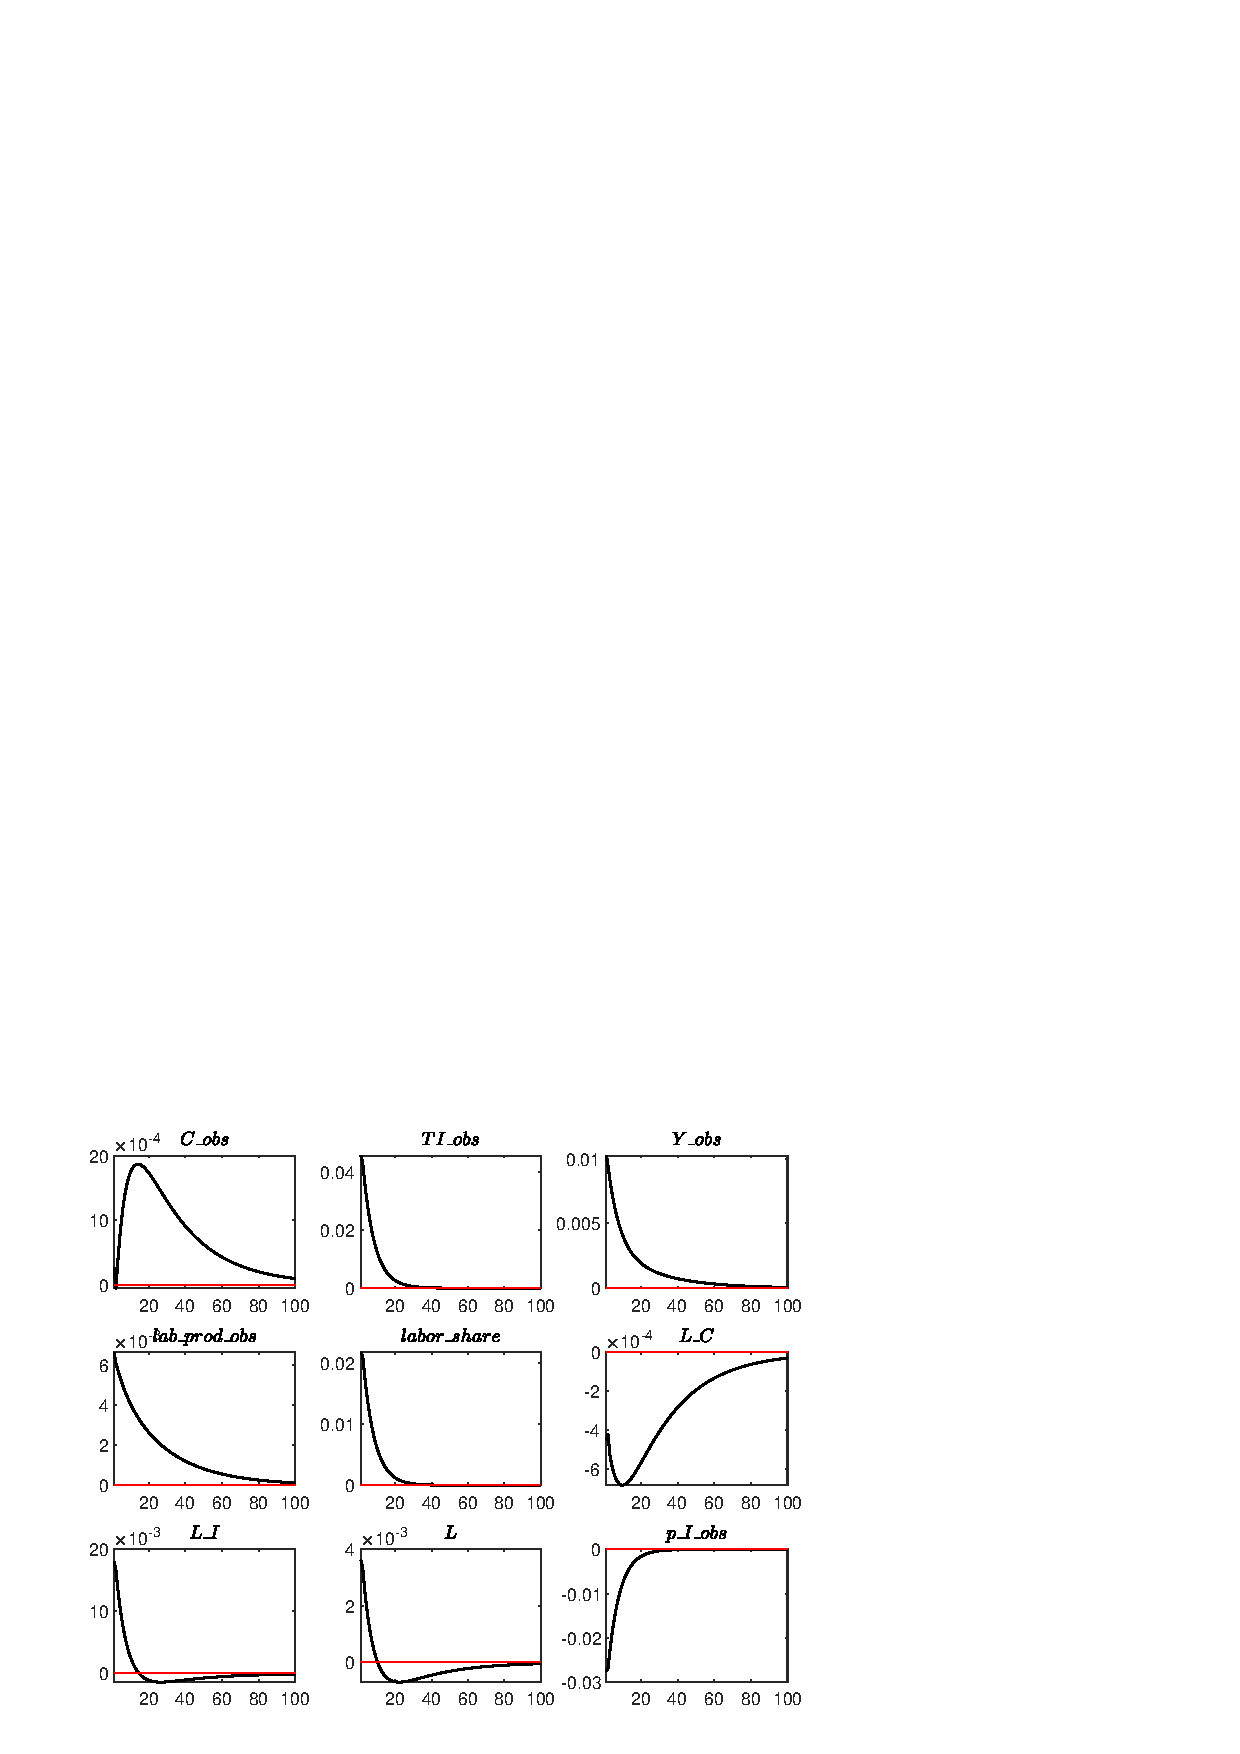
\includegraphics[width=0.80\textwidth]{directed_search_est/graphs/directed_search_est_IRF_e_ZI}
\caption{Impulse response functions (orthogonalized shock to $e\_ZI$).}
\label{Fig:IRF:e_ZI}
\end{figure}
 
\begin{figure}[H]
\centering 
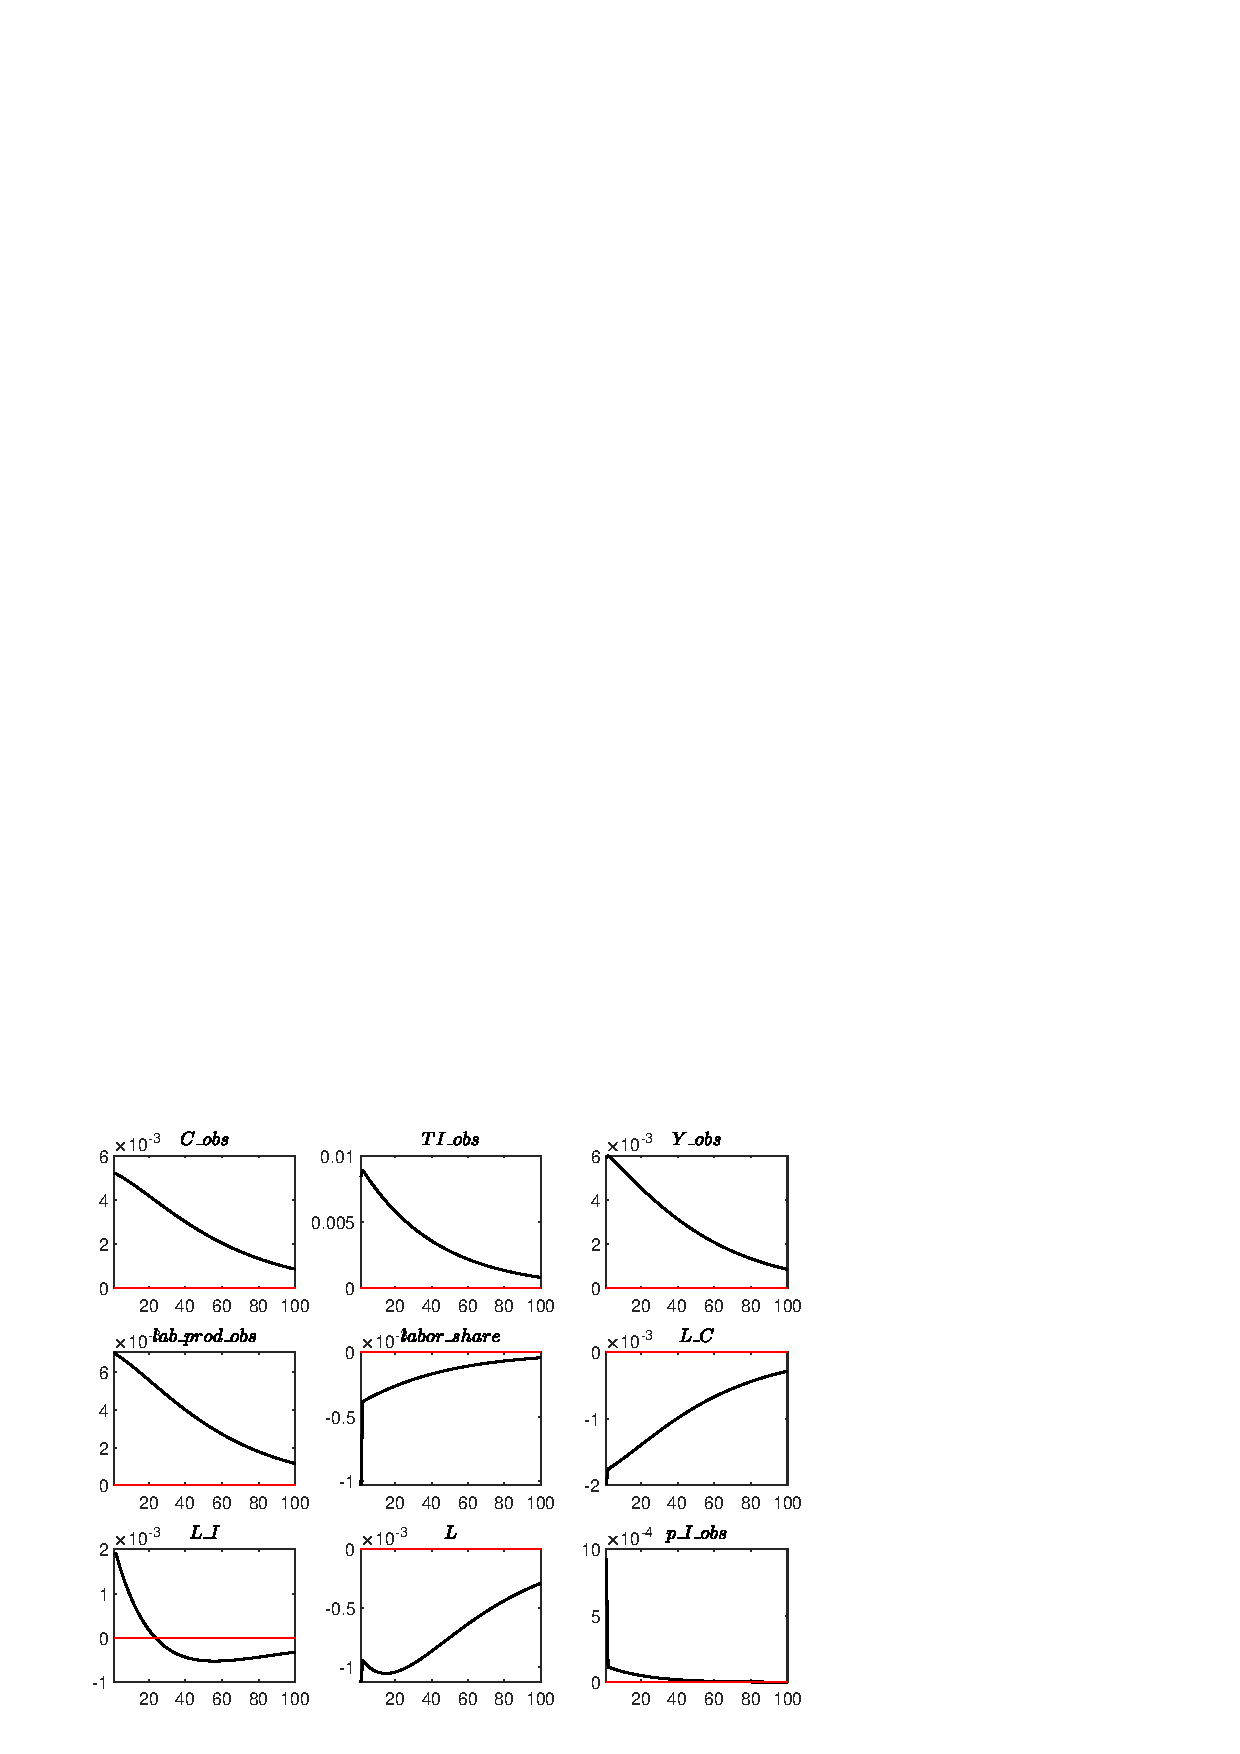
\includegraphics[width=0.80\textwidth]{directed_search_est/graphs/directed_search_est_IRF_e_Z}
\caption{Impulse response functions (orthogonalized shock to $e\_Z$).}
\label{Fig:IRF:e_Z}
\end{figure}
 
\begin{figure}[H]
\centering 
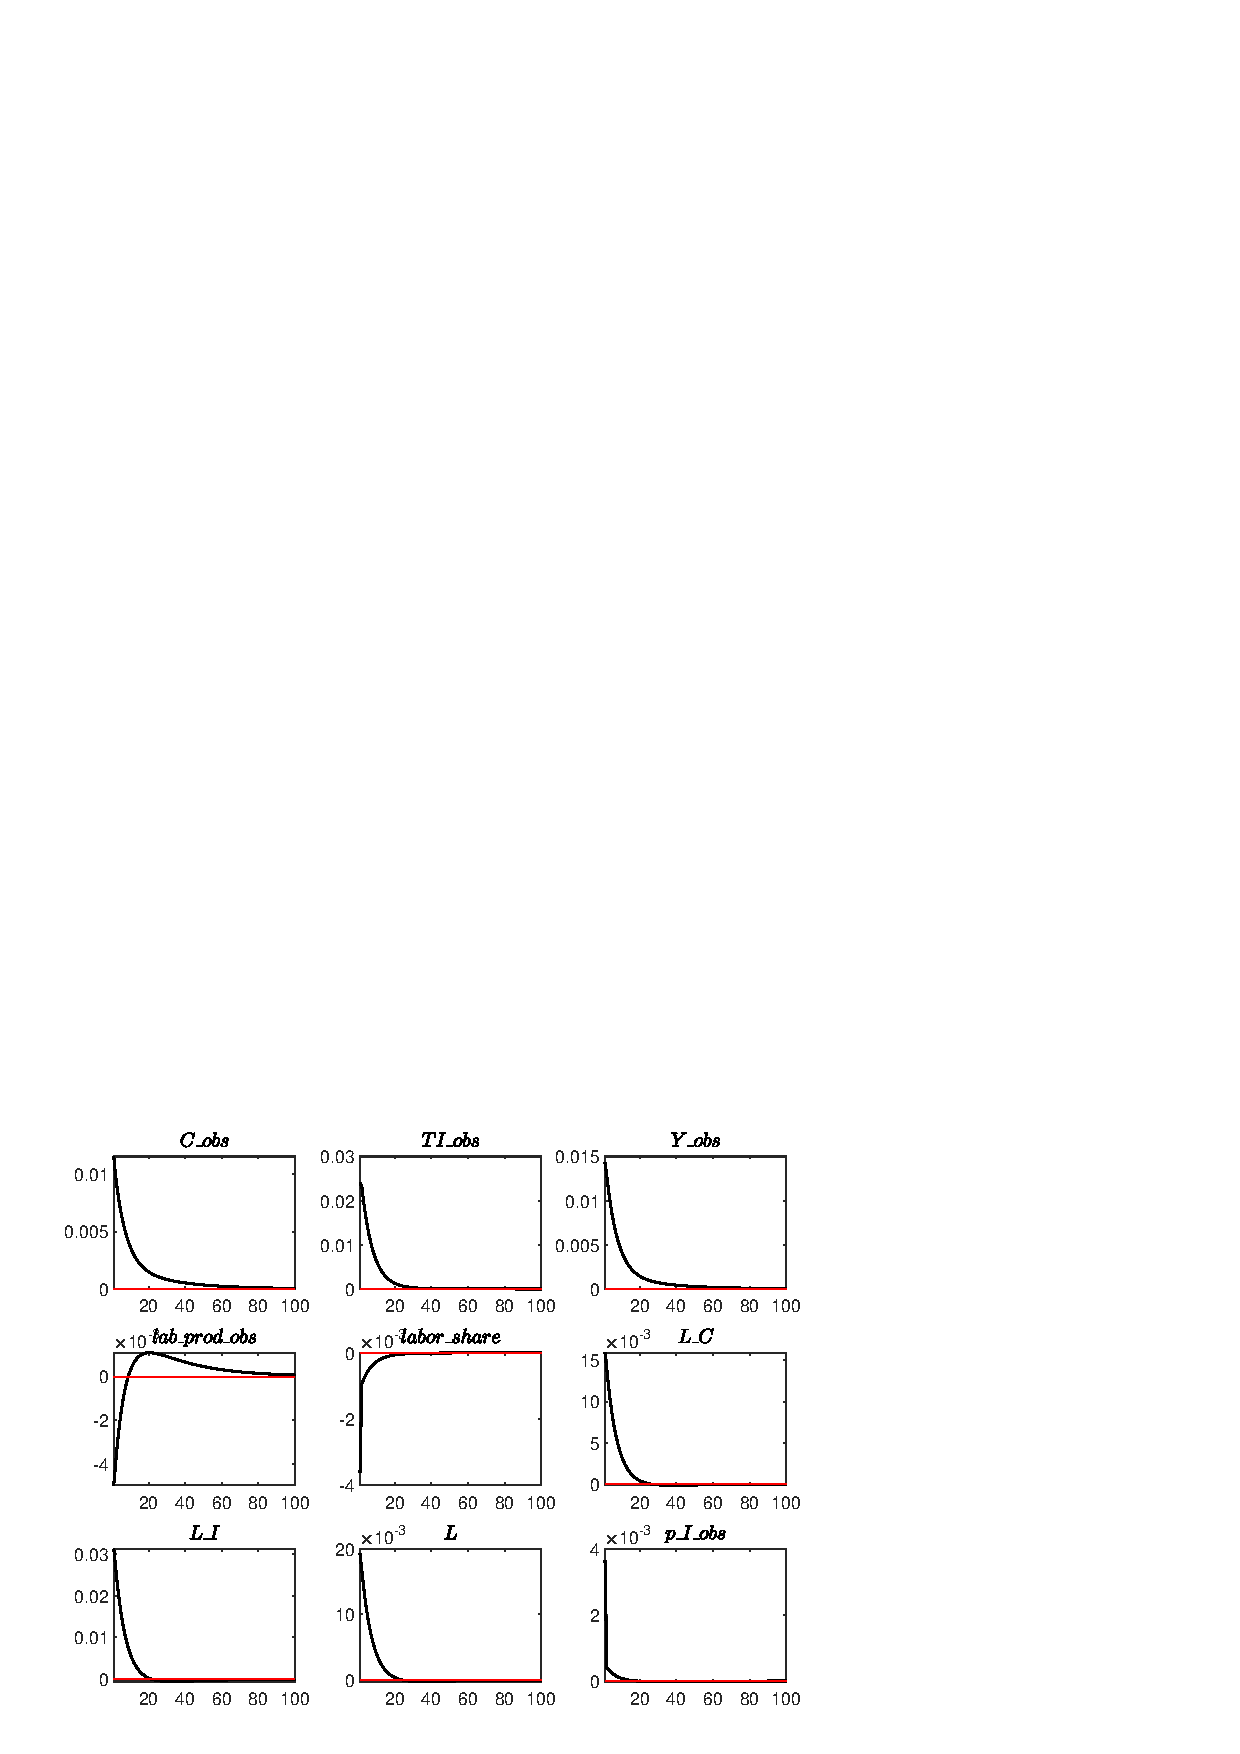
\includegraphics[width=0.80\textwidth]{directed_search_est/graphs/directed_search_est_IRF_e_chi}
\caption{Impulse response functions (orthogonalized shock to $e\_chi$).}
\label{Fig:IRF:e_chi}
\end{figure}
 
\begin{figure}[H]
\centering 
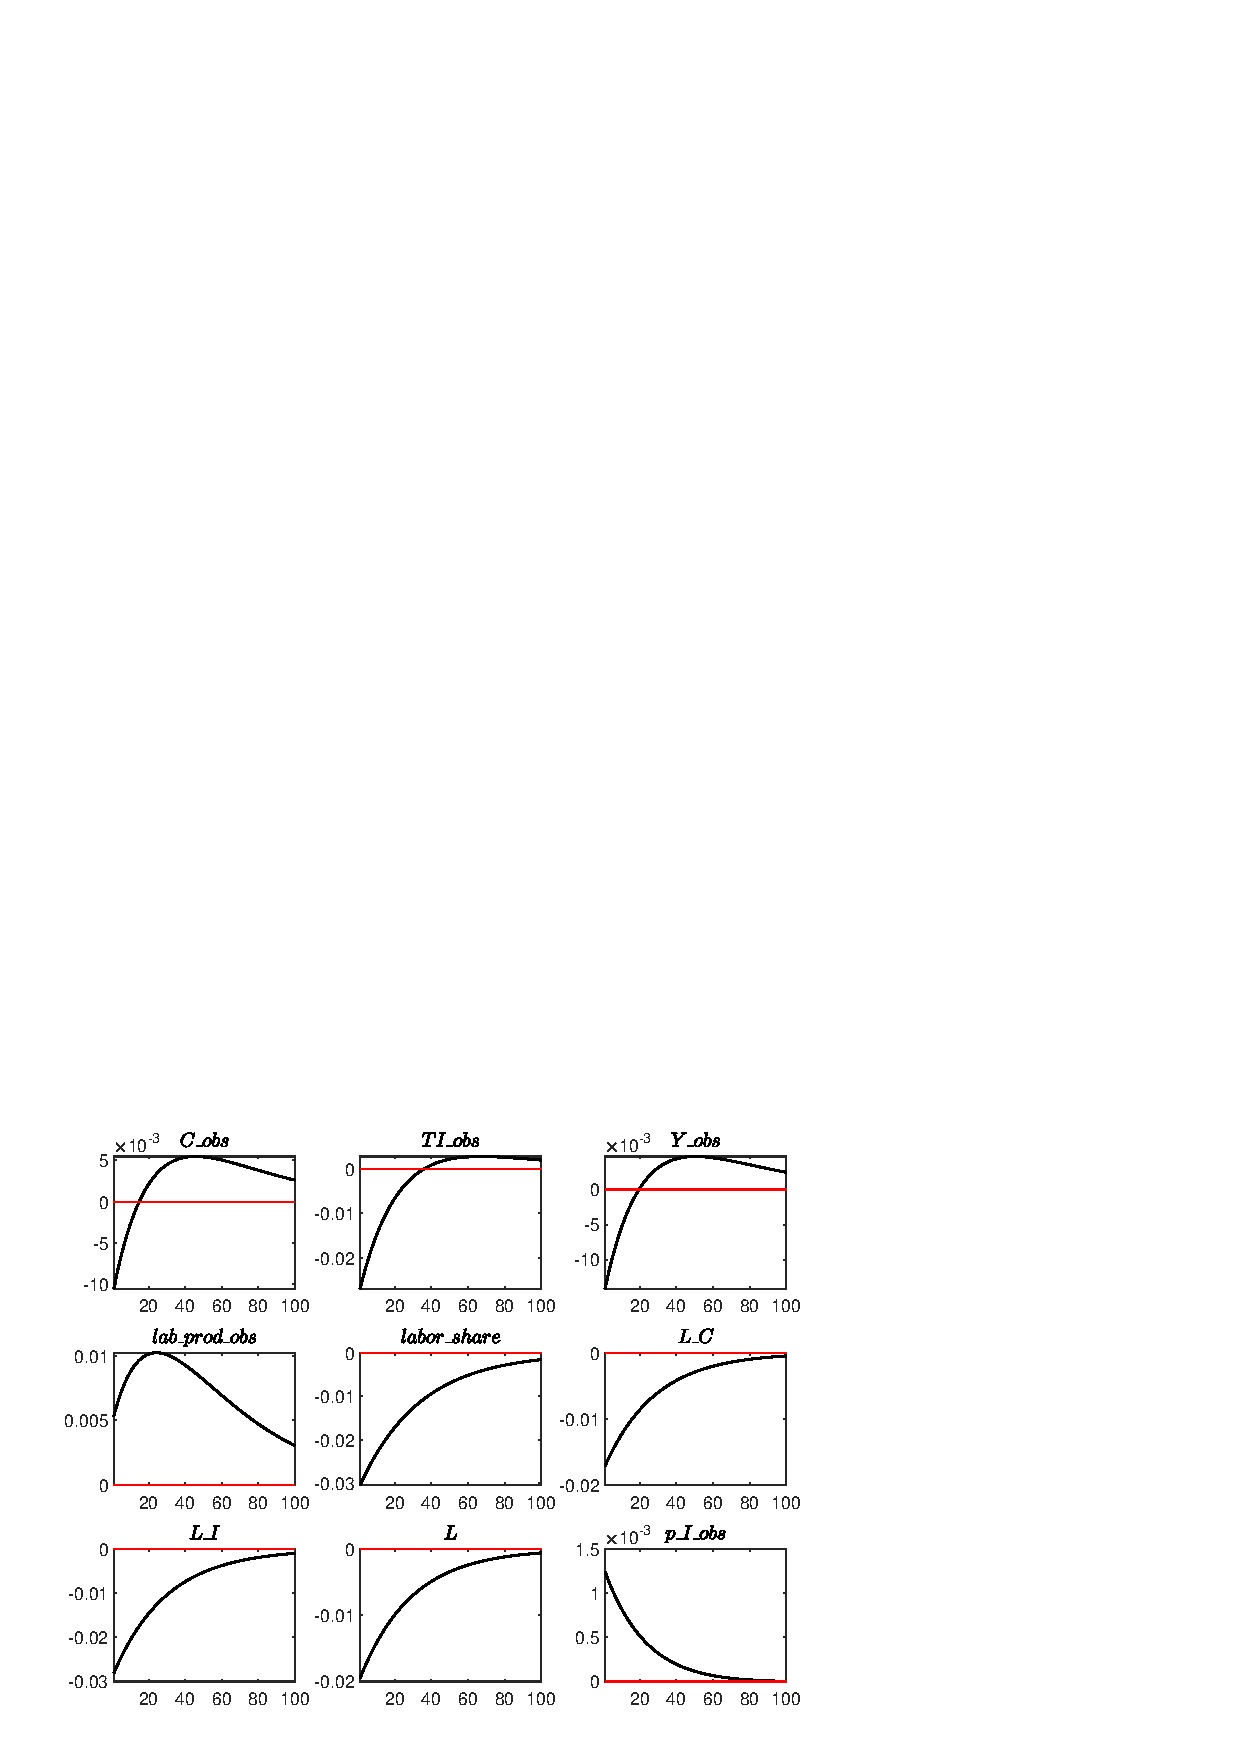
\includegraphics[width=0.80\textwidth]{directed_search_est/graphs/directed_search_est_IRF_e_kappa}
\caption{Impulse response functions (orthogonalized shock to $e\_kappa$).}
\label{Fig:IRF:e_kappa}
\end{figure}
 
\begin{figure}[H]
\centering 
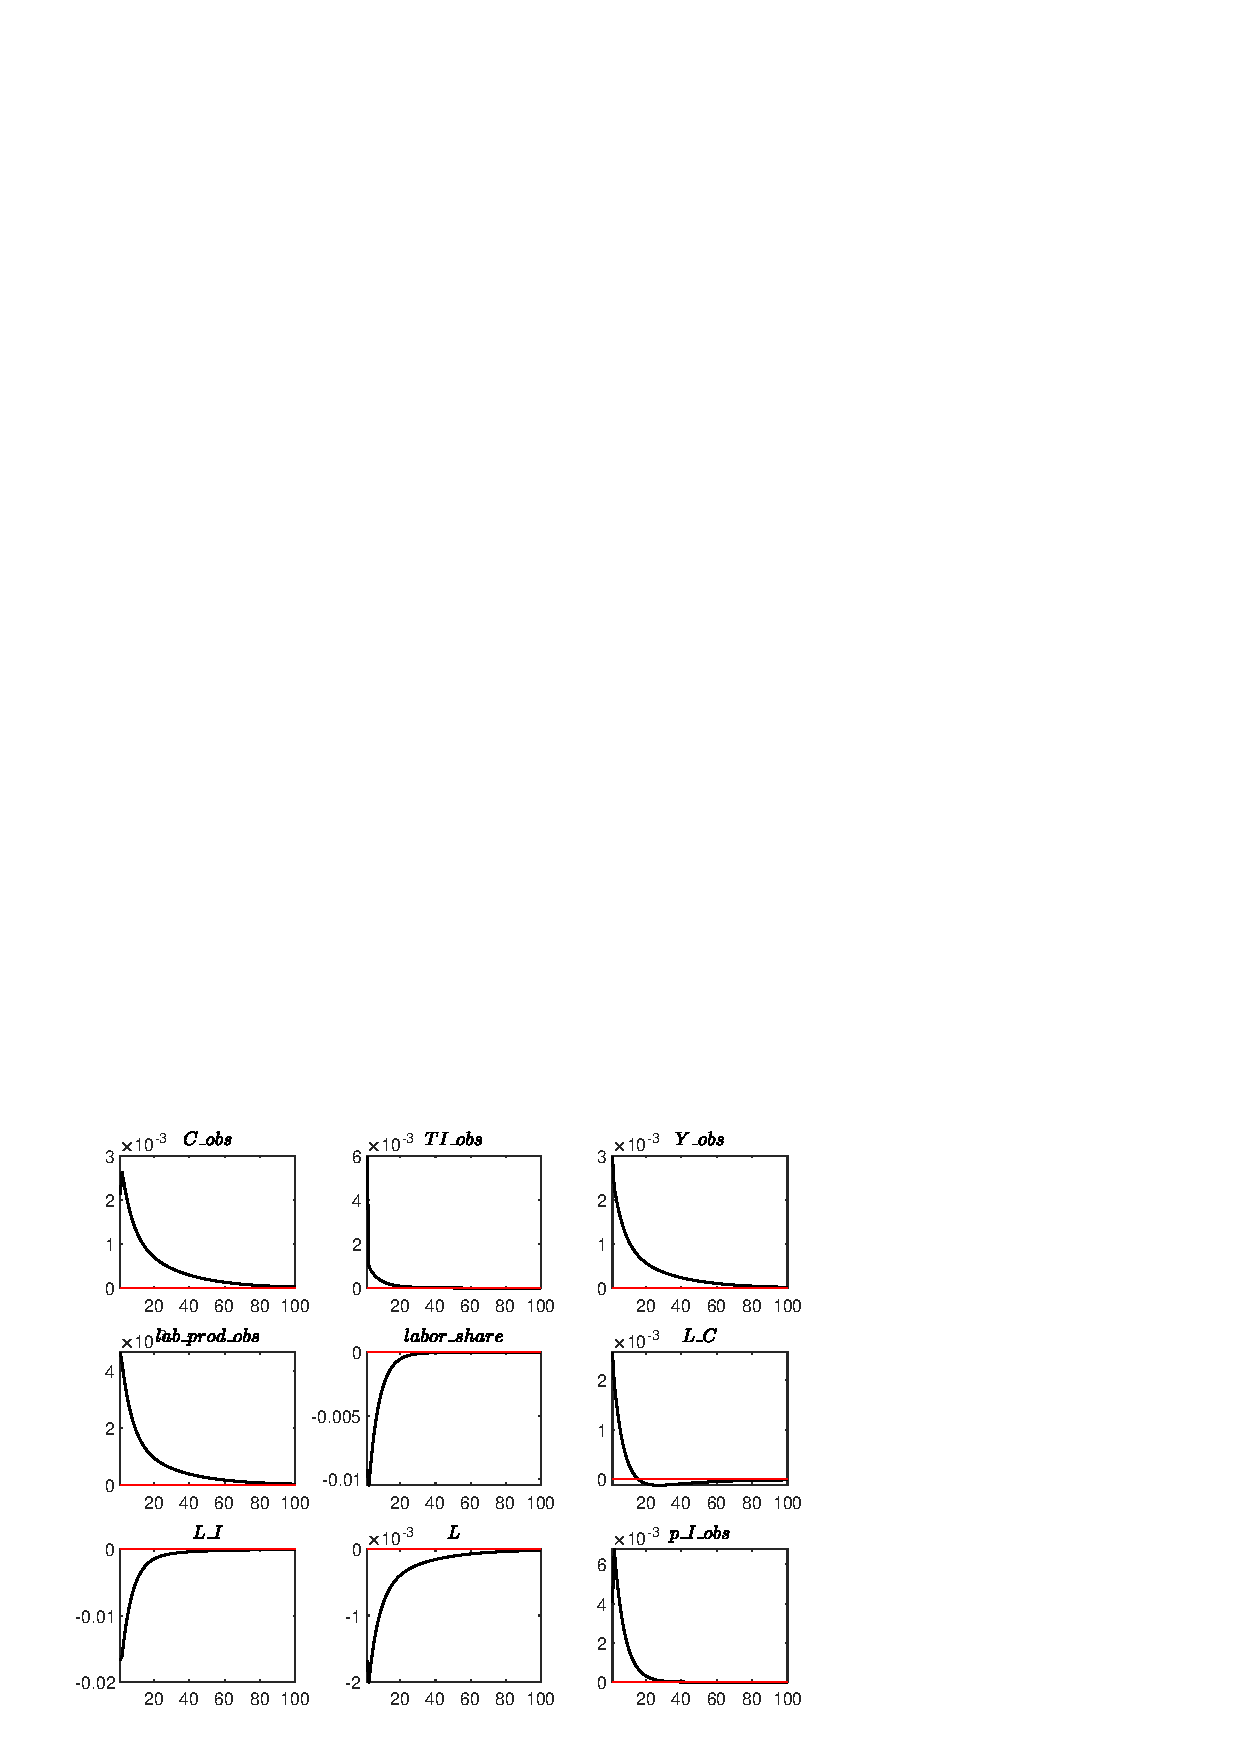
\includegraphics[width=0.80\textwidth]{directed_search_est/graphs/directed_search_est_IRF_e_zeta}
\caption{Impulse response functions (orthogonalized shock to $e\_zeta$).}
\label{Fig:IRF:e_zeta}
\end{figure}
 
 
% End Of TeX file. 
